For the first MAARSY data file the data time duration is approximately $34\,\si{\second}$. After compensating for the DC component in the complex data of each receiver, a coherent integration is applied to the timeseries data to improve the signal to noise ratio.\\

Further, the spectra of the individual receiver channels are calculated to obtain the magnitude and phase information vs frequency. Additionally, the cross spectra of the receiver pairs are calculated. These are the spectra of their cross-correlations. Since this is a form of convolution in time domain, one can obtain the cross spectrum by performing the multiplication of the individual receiver spectra in frequency domain (Convolution Theorem) \cite{conv_theorem}, albeit making sure that the second spectrum is in complex conjugate form (as seen earlier).\\

\begin{figure}
    \begin{center}
        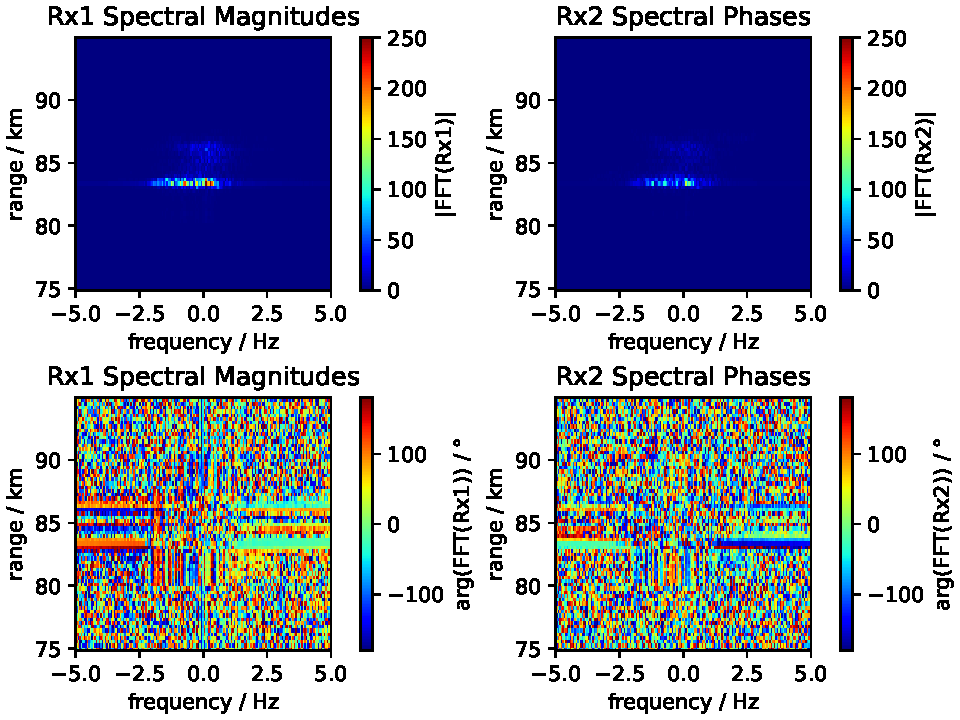
\includegraphics[width=0.8\textwidth]{graphics/t5/t5-reg-mag-phase.pdf}
    \end{center}
    \caption{Task 5: Magnitude and phase plots of the time series spectra of channels 1 and 2.}
    \label{fig:t5-mag-phase}
\end{figure}

\begin{figure}
    \begin{center}
        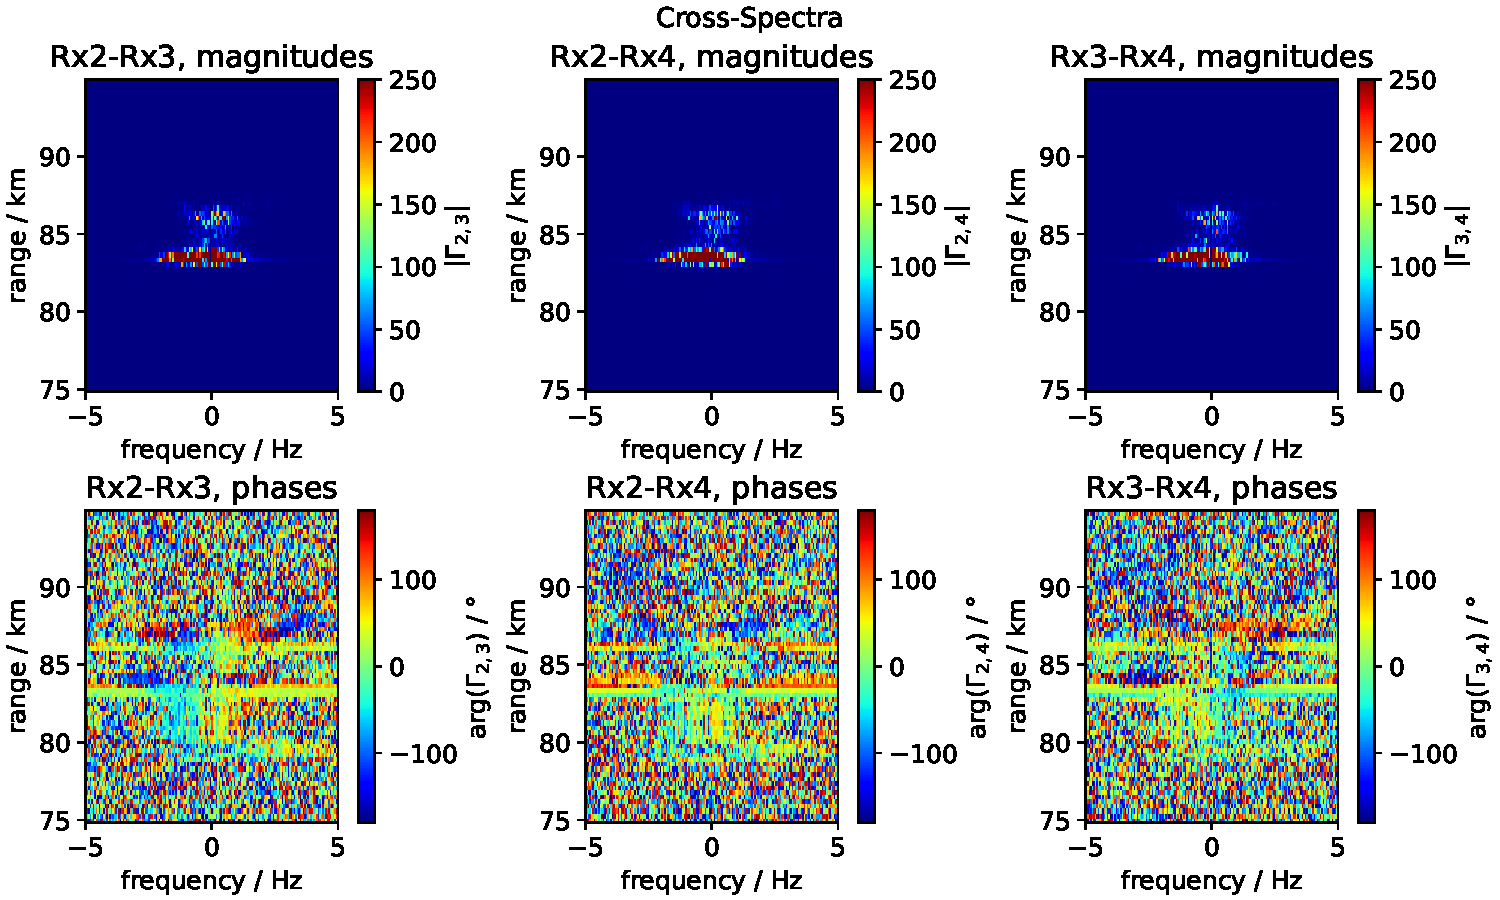
\includegraphics[width=\textwidth]{graphics/t5/t5-xspec-mag-phase.pdf}
    \end{center}
    \caption{Task 5: Magnitude and phase plots of the cross spectra of all receiver channels.}
    \label{fig:t5-xspec}
\end{figure}

The phases, seen in figures \ref{fig:t5-mag-phase} and \ref{fig:t5-xspec} are very noisy outside of the range gates of high SNR but some patterns are visible. In these larger SNR regions, the phase shows low variability. The data has been aquired recently and the echo power vs range shows that this might be a polar mesospheric summer echo (figure \ref{fig:t5-power}) \cite{pmse}.\\

The color range in figures \ref{fig:t5-mag-phase} and \ref{fig:t5-xspec} are the same. Therefore an increase in the signal to noise ratio after applying the cross spectrum calculation is visible.

\begin{figure}
    \begin{center}
        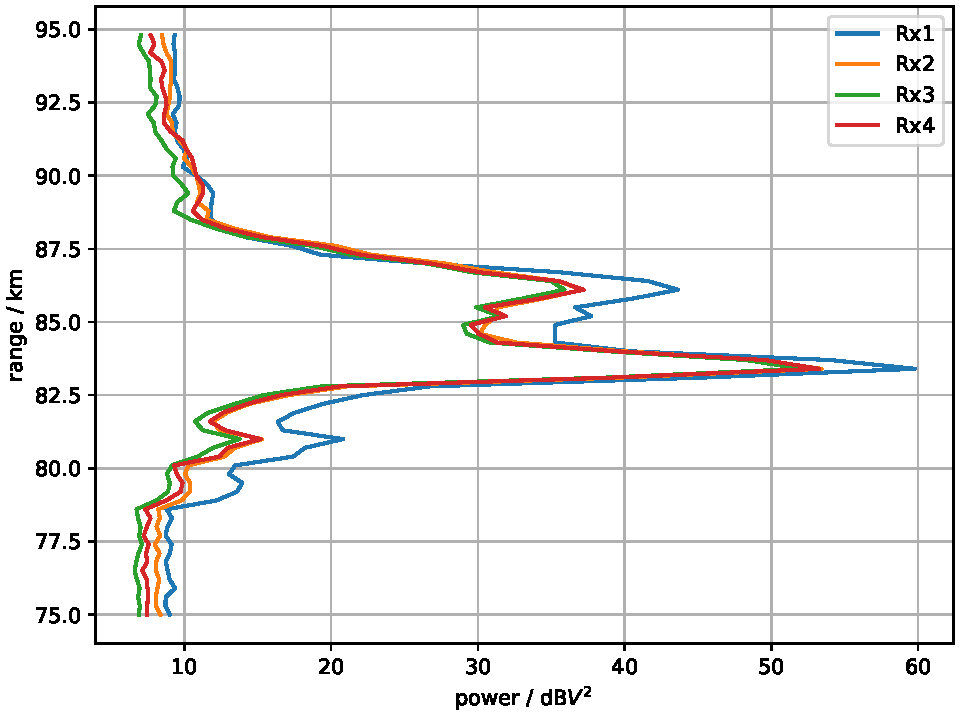
\includegraphics[width=0.62\textwidth]{graphics/t5/t5-power.pdf}
    \end{center}
    \caption{Task 5: Received power values over all range gates.}
    \label{fig:t5-power}
\end{figure}

% https://en.wikipedia.org/wiki/Polar_mesospheric_summer_echoes

